\documentclass[11pt,a4paper]{article}

\usepackage[utf8]{inputenc}
\usepackage[T1]{fontenc}
\usepackage[spanish]{babel}
\usepackage{amsmath,amssymb}
\usepackage{graphicx}
\usepackage{booktabs}
\usepackage[margin=2.5cm]{geometry}
\usepackage[colorlinks=true, linkcolor=black, urlcolor=blue]{hyperref}
% Marca visible para lo que falta por completar
\newcommand{\pendiente}[1]{\textbf{[PENDIENTE: #1]}}

% Inserta una imagen si existe; si no, muestra un aviso (el informe compila igual)
\newcommand{\hoja}[2]{%
  \IfFileExists{#1}
    {\includegraphics[width=#2\textwidth]{#1}}
    {\fbox{\parbox{0.8\textwidth}{\centering
      \pendiente{falta el archivo \texttt{#1}}}}}%
}

\title{Práctica 2: Multiplicación rápida de enteros\\
Algoritmo de Karatsuba}

\author{José Eduardo Piña Montero \and Angel David Quimbayo Carvajal}

\date{Análisis y Diseño de Algoritmos \\ \today}

\begin{document}
\maketitle

\section{Deducción de la identidad de Karatsuba}

\subsection{El método clásico y por qué es cuadrático}

Sean $x$ e $y$ dos enteros de $n$ dígitos en base $B$, y sea $m = n/2$.
Partimos cada número en su mitad alta y su mitad baja:
\[
  x = x_1 B^m + x_0, \qquad y = y_1 B^m + y_0,
\]
donde $0 \le x_0, y_0 < B^m$. Multiplicando y distribuyendo:
\begin{align}
  x \cdot y & = (x_1 B^m + x_0)(y_1 B^m + y_0) \notag                                 \\
            & = x_1 y_1 B^{2m} + (x_1 y_0 + x_0 y_1) B^m + x_0 y_0. \label{eq:cuatro}
\end{align}
Esta expresión requiere \emph{cuatro} productos de números de $m = n/2$ dígitos: $x_1y_1$, $x_1y_0$, $x_0y_1$ y $x_0y_0$. El resto del trabajo (sumas y desplazamientos por potencias de $B$) es lineal en $n$. Por tanto
\[
  T(n) = 4\,T(n/2) + \Theta(n),
\]
que no mejora el orden cuadrático del método del colegio.

\subsection{La observación de Karatsuba}

De los cuatro productos de \eqref{eq:cuatro}, los extremos $x_1y_1$ y $x_0y_0$
son necesarios. Pero del producto central solo nos interesa la \emph{suma}
$x_1y_0 + x_0y_1$, no cada sumando por separado. La idea es obtener esa suma
con un único producto adicional. Definimos
\[
  P_1 = x_1 y_1, \qquad P_2 = x_0 y_0, \qquad P_3 = (x_1 + x_0)(y_1 + y_0).
\]
Desarrollando $P_3$:
\[
  P_3 = x_1 y_1 + x_1 y_0 + x_0 y_1 + x_0 y_0 = P_1 + (x_1 y_0 + x_0 y_1) + P_2 .
\]
Despejando el término central:
\begin{equation}
  x_1 y_0 + x_0 y_1 = P_3 - P_1 - P_2. \label{eq:central}
\end{equation}
Sustituyendo \eqref{eq:central} en \eqref{eq:cuatro} obtenemos la identidad de Karatsuba:
\begin{equation}
  \boxed{\,x \cdot y = P_1 B^{2m} + (P_3 - P_1 - P_2) B^m + P_2\,} \label{eq:karatsuba}
\end{equation}

\subsection{Por qué tres productos y no cuatro}

El producto $P_3$ ``contiene'' a la vez los dos productos cruzados que antes
calculábamos por separado, junto con $P_1$ y $P_2$, que ya teníamos. Como $P_1$
y $P_2$ se necesitan de todos modos, restarlos de $P_3$ deja exactamente
$x_1y_0 + x_0y_1$. Hemos cambiado un producto recursivo de $m$ dígitos por dos
sumas y tres restas de números de a lo sumo $n$ dígitos, que cuestan
$\Theta(n)$ y no aumentan el orden del término no recursivo. Así la recurrencia
pasa de $4T(n/2)+\Theta(n)$ a
\[
  T(n) = 3\,T(n/2) + \Theta(n).
\]

\subsection{Detalles que importan en la implementación}

\begin{itemize}
  \item \textbf{Dígito adicional.} Las sumas $x_1 + x_0$ e $y_1 + y_0$ pueden tener $m+1$ dígitos. Eso no cambia el orden lineal del término no recursivo, pero obliga a que las funciones auxiliares admitan operandos y resultados de longitud variable.
  \item \textbf{Orden de las restas.} El término central es no negativo, pero para evitar un negativo intermedio con dígitos sin signo se calcula primero $P_3 - P_1$ y luego se resta $P_2$. Ambas restas son no negativas, porque
        \[
          P_3 - P_1 = P_2 + x_1 y_0 + x_0 y_1 \ge P_2 .
        \]
\end{itemize}

\subsection{Ejemplo numérico}

Sea $x = 1234$, $y = 5678$, $B = 10$, $m = 2$. Entonces $x_1 = 12$, $x_0 = 34$,
$y_1 = 56$, $y_0 = 78$ y
\begin{align*}
  P_1 & = 12 \cdot 56 = 672,                    \\
  P_2 & = 34 \cdot 78 = 2652,                   \\
  P_3 & = (12+34)(56+78) = 46 \cdot 134 = 6164.
\end{align*}
El término central es $P_3 - P_1 - P_2 = 6164 - 672 - 2652 = 2840$, que coincide con $x_1y_0 + x_0y_1 = 12\cdot 78 + 34 \cdot 56 = 936 + 1904 = 2840$. Por la identidad \eqref{eq:karatsuba}:
\[
  x \cdot y = 672 \cdot 10^4 + 2840 \cdot 10^2 + 2652 = 7\,006\,652,
\]
que es el valor de $1234 \cdot 5678$.

\pagebreak

\section{Resolución de la recurrencia $T(n) = 3T(n/2) + \Theta(n)$}

% Esta sección se desarrolla a mano (Teorema Maestro y árbol de recurrencia).
% Para incluirla: escanear/fotografiar las hojas, guardarlas en informe/img/
% como recurrencia1.png, recurrencia2.png, ... y ajustar la cantidad de figuras.

\begin{figure}[h!]
  \centering
  \hoja{img/Resolucion_recurrencia.png}{0.65}
  \caption{Resolución de la recurrencia: Teorema Maestro \& Árbol de recurrencia.}
\end{figure}

\section{Análisis experimental}

\subsection{Montaje}
Las mediciones se hicieron en un MacBook Air con procesador Apple M1 y macOS,
compilando con Apple clang 21.0.0 (\texttt{c++ -std=c++17 -O2 -Wall -Wextra}) y
sin \texttt{-flto}, de modo que el compilador no puede ver a través de las
llamadas a los algoritmos ni eliminar el cálculo. El reloj es
\texttt{std::chrono::steady\_clock}.

Se midieron tamaños $n = 2, 4, 8, \dots, 4096$ dígitos. Para cada $n$ se
generan dos operandos aleatorios de exactamente $n$ dígitos, con semilla fija,
y ambos algoritmos reciben los mismos números. Antes de medir, se comprueba
(fuera de la zona cronometrada) que los dos algoritmos dan el mismo producto.
Para cada algoritmo y tamaño se hace una ejecución de calentamiento y luego se
calibra el número de repeticiones hasta que un lote dure al menos 100~ms, muy
por encima de la resolución del reloj. Se miden 7 lotes y se reporta la mediana
del tiempo por multiplicación. Cada resultado se consume (se acumulan su
longitud y su último dígito, que se imprime al final) para evitar que el
cálculo se elimine.

Karatsuba se midió con distintos umbrales del caso base: con \texttt{UMBRAL}
$=u$, los operandos de a lo sumo $u$ dígitos se multiplican con el método
clásico. Con $u=1$ la recursión llega hasta un dígito (Karatsuba ``puro''); con
$u > 1$ se obtiene una versión híbrida. Se usaron $u \in \{1, 16, 64, 128\}$ en
dos corridas completas y $u \in \{256, 512\}$ en una tercera.

Una limitación: la medición no se hizo sobre un sistema dedicado, sino sobre
macOS, que mantiene procesos en segundo plano y no permite fijar el proceso a
un núcleo. Entre las dos corridas completas las diferencias son de alrededor de
1\% o menos en los tamaños grandes, y llegan a cerca de 8\% en algunos tamaños
pequeños; por eso los casos en que la ventaja es muy pequeña se reportan como
empates.

\subsection{Resultados}
La Tabla~\ref{tab:tiempos} muestra el tiempo medio por multiplicación y la
Figura~\ref{fig:tiempo} lo grafica en escala log-log.

\begin{table}[h!]
  \centering\footnotesize
  \setlength{\tabcolsep}{4pt}
  \begin{tabular}{rrrrrrrr}
    \toprule
    $n$  & Clásica & K$_{1}$  & K$_{16}$ & K$_{64}$ & K$_{128}$ & K$_{256}$ & K$_{512}$ \\
    \midrule
    2    & 0.0585  & 0.552    & 0.065    & 0.065    & 0.066     & 0.064     & 0.065     \\
    4    & 0.0735  & 3.13     & 0.083    & 0.083    & 0.083     & 0.081     & 0.083     \\
    8    & 0.151   & 11.0     & 0.166    & 0.166    & 0.166     & 0.163     & 0.166     \\
    16   & 0.297   & 37.1     & 0.329    & 0.328    & 0.322     & 0.315     & 0.307     \\
    32   & 0.609   & 119      & 3.21     & 0.706    & 0.706     & 0.772     & 0.694     \\
    64   & 2.07    & 368      & 13.4     & 1.85     & 1.85      & 1.82      & 1.85      \\
    128  & 6.62    & 1\,170   & 47.9     & 11.4     & 6.97      & 6.58      & 6.69      \\
    256  & 23.8    & 3\,340   & 141      & 38.3     & 27.3      & 23.6      & 23.6      \\
    512  & 86.4    & 10\,861  & 499      & 159      & 105       & 84.1      & 86.7      \\
    1024 & 337     & 32\,415  & 1\,498   & 487      & 335       & 274       & 285       \\
    2048 & 1\,339  & 99\,886  & 4\,798   & 1\,646   & 1\,115    & 913       & 877       \\
    4096 & 5\,367  & 297\,688 & 14\,316  & 4\,945   & 3\,391    & 2\,796    & 2\,738    \\
    \bottomrule
\end{tabular}
  \caption{Tiempo medio por multiplicación (\textmu s) en macOS (Apple M1).
    K$_u$ es Karatsuba con UMBRAL $=u$. Mediana entre dos corridas
    (una sola corrida para $u=256$ y $u=512$).}
  \label{tab:tiempos}
\end{table}

\begin{figure}[h!]
  \centering
  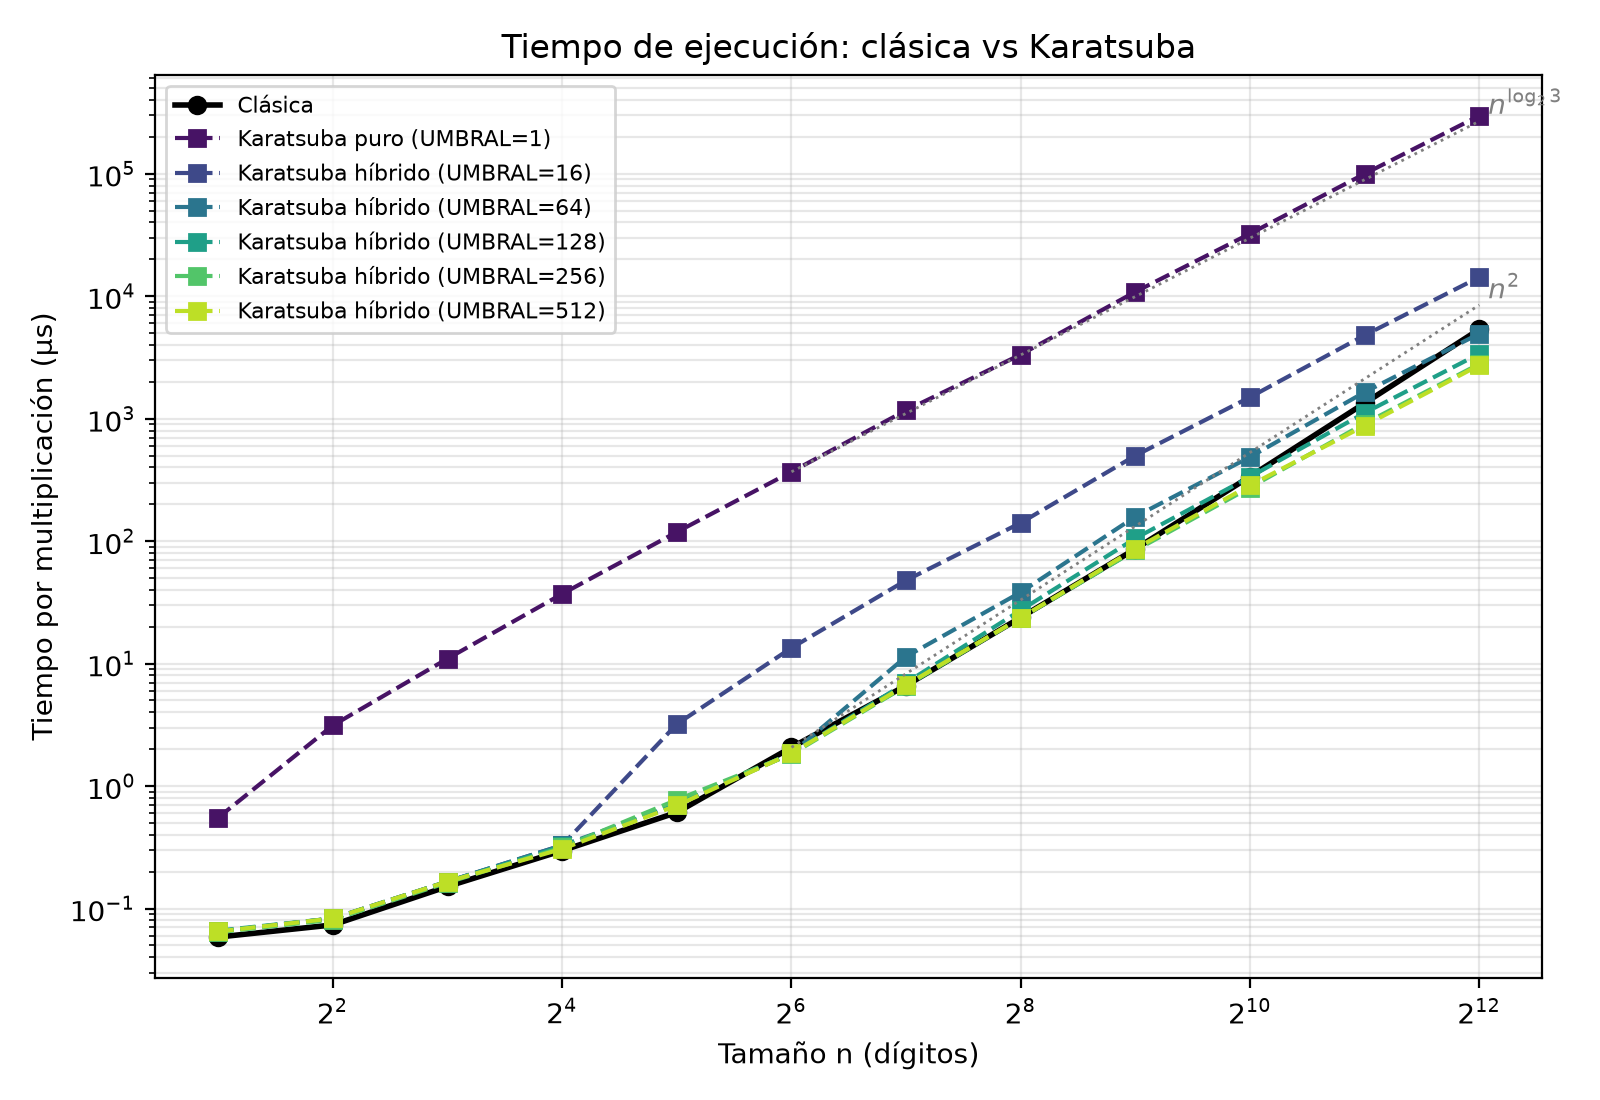
\includegraphics[width=0.65\textwidth]{../docs/macos_tiempo.png}
  \caption{Tiempo frente al tamaño, en escala log-log. Las rectas punteadas
    son las pendientes de $n^2$ y de $n^{\log_2 3}$.}
  \label{fig:tiempo}
\end{figure}

\subsection{Punto de cruce}
Definimos la razón $r(n) = T_{\text{clásica}}(n) / T_{\text{Karatsuba}}(n)$: si
$r > 1$, Karatsuba es más rápido. El punto de cruce es el menor $n > u$ desde
el cual $r > 1$ para todos los tamaños mayores. Se excluyen los $n \le u$
porque ahí Karatsuba ejecuta el mismo caso base cuadrático que la clásica, y
cualquier diferencia viene del código y no del algoritmo. El resultado depende
del umbral (Tabla~\ref{tab:cruce} y Figura~\ref{fig:razon}).

\begin{table}[h!]
  \centering\small
  \begin{tabular}{rcl}
    \toprule
    \texttt{UMBRAL} & $r(4096)$ & Punto de cruce                     \\
    \midrule
    1 (puro)        & 0.018     & no aparece en el rango medido      \\
    16              & 0.375     & no aparece en el rango medido      \\
    64              & 1.085     & $n = 4096$ (ventaja de 8\%)        \\
    128             & 1.59      & entre 1024 y 2048 (empate en 1024) \\
    256             & 1.90      & entre 512 y 1024 (empate en 512)   \\
    512             & 1.96      & $n = 1024$                         \\
    \bottomrule
  \end{tabular}
  \caption{Razón $r$ a 4096 dígitos y punto de cruce según el umbral.}
  \label{tab:cruce}
\end{table}

Con $u=1$ y $u=16$ no hay cruce dentro de 2 a 4096 dígitos, pero $r$ crece unas
1.3 veces por cada duplicación de $n$, que es lo esperado: $n^2 / n^{\log_2 3}
  = n^{0.415}$ y $2^{0.415} \approx 1.33$. Extrapolando, el cruce estaría en el
orden de decenas de miles de dígitos para $u=16$ y de decenas de millones para
$u=1$ (es una extrapolación, no una medición). Con umbrales de 128 o más el
cruce sí aparece dentro del rango. En $u=128$ y $u=256$ la ventaja en el primer
tamaño es de menos de 2\%, así que se trata de empates y no de cruces firmes.
Los mejores resultados se obtienen con $u$ entre 256 y 512, donde Karatsuba es
unas 1.9 veces más rápido a 4096 dígitos.

\begin{figure}[h!]
  \centering
  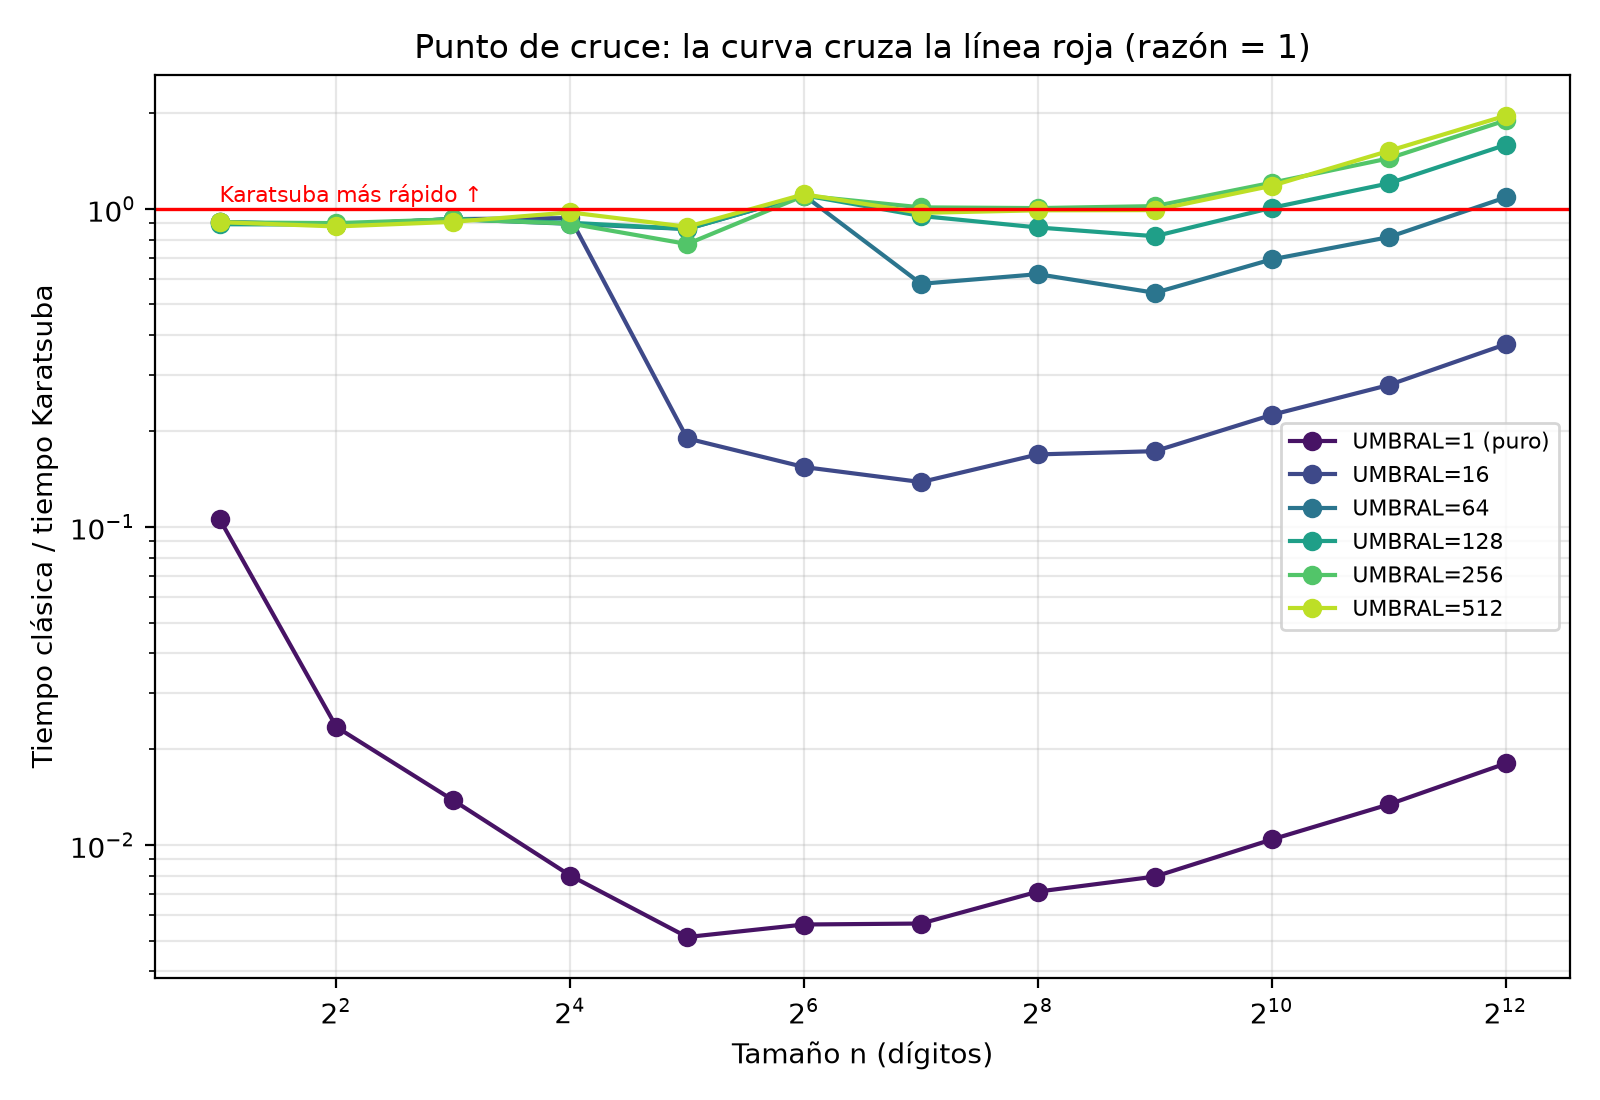
\includegraphics[width=0.65\textwidth]{../docs/macos_razon.png}
  \caption{Razón entre el tiempo de la clásica y el de Karatsuba. Donde la
    curva supera la línea roja, Karatsuba es más rápido.}
  \label{fig:razon}
\end{figure}

\subsection{Complejidad asintótica frente a rendimiento real}
Los datos confirman la cota asintótica. Al duplicar $n$, el tiempo de la
clásica se multiplica por $\approx 4$ y el de Karatsuba puro por $\approx 3$;
los exponentes ajustados por mínimos cuadrados sobre $n \ge 128$ son $1.94$
para la clásica y $1.61$ para Karatsuba puro, frente a $2$ y $\log_2 3 \approx
  1.585$ (Figura~\ref{fig:tiempo}). Sin embargo, la cota asintótica describe cómo
crece el tiempo, no cuál es más rápido para un tamaño concreto: las constantes
ocultas deciden el rango en que cada método gana.

\textbf{Constantes ocultas.} La clásica es un doble ciclo sobre enteros con
acceso contiguo a memoria; a 4096 dígitos cuesta unos
$5367\,\mu\text{s}/4096^2 \approx 0.32$~ns por producto de dígitos. En cambio, el
trabajo lineal de cada llamada recursiva de Karatsuba (partir, rellenar, sumar,
restar y desplazar cadenas) crea y copia una veintena de cadenas de tamaño
cercano a $n$. Esas copias y asignaciones de memoria son $\Theta(n)$ y no
cambian el orden asintótico, pero su constante es mucho mayor que la del ciclo
clásico. Karatsuba puro a 4096 dígitos tarda unos 298\,000~$\mu$s, unas 55
veces el tiempo de la clásica.

\textbf{Un modelo simple.} Un nivel de recursión ahorra unos $\tfrac14 c_0 n^2$
(la clásica hace 4 subproductos de tamaño $n/2$ y Karatsuba 3) y añade unos
$c_1 n$ de trabajo lineal. Compensa cuando $n \gtrsim 4c_1/c_0$. Con
$c_0 \approx 0.32$~ns y un cruce observado entre 512 y 1024, resulta $c_1$ del
orden de decenas de nanosegundos por dígito, más de cien veces $c_0$. Es una
estimación de orden de magnitud, no una medición directa.

\textbf{El salto en $n = 2u$.} Con $u=16$, la razón es $\approx 0.9$ en $n=16$
(mismo caso base) y cae a $0.19$ en $n=32$: un solo nivel de recursión cuesta
unas cinco veces lo que cuesta la multiplicación clásica completa a ese tamaño.
Una posible causa adicional (hipótesis, no comprobada) es que las sumas
$x_1+x_0$ pueden tener $m+1$ dígitos, superar el umbral y provocar un nivel
extra de recursión.

Por eso el umbral importa: delegar los tamaños pequeños en el ciclo clásico
evita pagar la sobrecarga de la recursión donde no compensa. Esto explica por
qué para números pequeños el método clásico puede ser más rápido aunque su
complejidad asintótica sea peor.

\section{Conclusiones y dificultades encontradas}

\subsection{Conclusiones}
\pendiente{Resumir lo aprendido sobre la identidad, la recurrencia y los resultados experimentales.}

\subsection{Dificultades}
\pendiente{Describir problemas reales que tuvieron (implementación, medición, herramientas) y cómo los resolvieron.}

\section*{Declaración de uso de inteligencia artificial}

\pendiente{Agregar declaración sobre el uso de inteligencia artificial en el desarrollo del informe.}

\end{document}